\ylDisplay{Pirnid} % Ülesande nimi
{Tundmatu autor} % Autor
{piirkonnavoor} % Voor
{2009} % Aasta
{P 7} % Ülesande nr.
{2} % Raskustase
{
% Teema: Elektriõpetus

\ifStatement
Urmol oli neli pirni, neist kolm uhesugused. Kui Urmo ühendas pirnid joonisel kujutatud viisil tundmatu pingeallikaga, põlesid nad kõik sama võimsusega. Pirnil 1 oli kirjas ”$10$ $W$”. Mis oli kirjas pirnidel $2$, kui on teada, et kõik pirnid on sama nimipingega? Lambi takistuse sõltuvusega temperatuurist mitte arvestada.
\begin{center}
	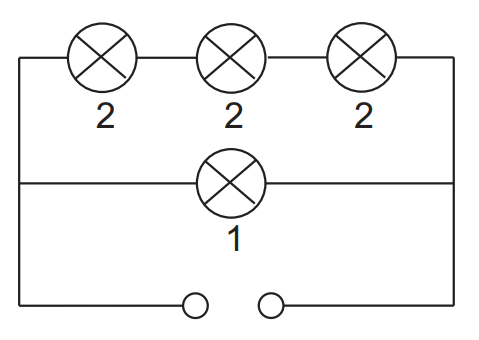
\includegraphics[width=0.5\linewidth]{2009-v2p-07-yl.png}
\end{center}
\fi

\ifHint
Võrdse nimipinge korral on nimivõimsused takistusega pöördvõrdelised.
\fi

\ifSolution
Olgu pirni 1 takistus $R_1$, pirni 2 takistus $R_2$ ja pingeallika pinge $U$. Siis pirni 1 pinge on $U$ ja pirnidel 2 igaühel pinge $U/3$. Teades, et 
$\frac{U^2}{R_1} = \frac{(U/3)^2}{R_2}$,
saame, et $R_1 = 9 R_2$. Võrdse nimipinge korral on nimivõimsused takistusega pöördvõrdelised, järelikult $P_2 = 9P_1 = 90 W$.
\fi
}